
\subsection{Sensores}
	\subsubsection{SHT31-SHT21}
	SHT31 es un sensor digital de temperatura y humedad relativa. Posee protocolo I2C.
	\paragraph*{Especificaciones}
	\begin{wrapfigure}{r}{0.4\linewidth}
		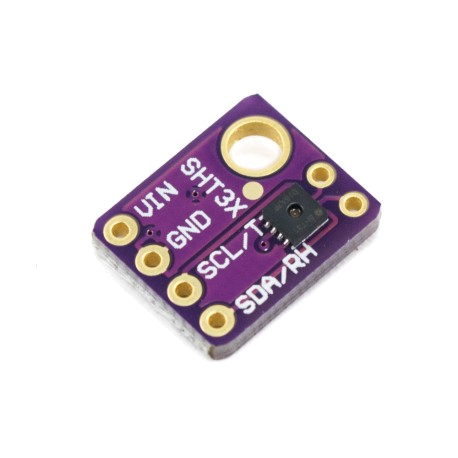
\includegraphics[scale=0.35]{SHT31.png}
		\caption{Placa SHT31}
		\label{fig:SHT31}
	\end{wrapfigure}
		\begin{itemize}
			\item   Voltaje de operación: 2.4 V a 5.5 V.
			\item	Rango de temperatura: -40\grad C a 12\grad C.
			\item   Resolución de temperatura: 0.015\grad C
			\item	Precisión de temperatura: 0.2\grad C 
			\item	Rango de humedad: 0 a 100\% RH
			\item   Resolución HR: 0.01 \% RH
			\item   Precisión HR: 2\% RH
			\item Frecuencia de muestreo: 157 Hz.
		\end{itemize}

	
	\subsubsection{BME280}
	BME280 es un dispositivo que mide presión atmosférica, temperatura y humedad relativa, con gran precisión, bajo consumo y compacto. Utiliza protocolo I2C para su comunicación.

	
	\begin{wrapfigure}{r}{0.4\linewidth}
		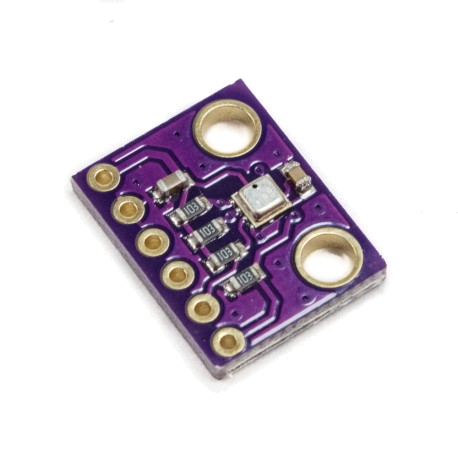
\includegraphics[width=0.4\textwidth]{bme280.png}
		\caption{Placa BME280}
		\label{fig:BME280}
	\end{wrapfigure}
		\paragraph*{Especificaciones}
		\begin{itemize}
		\item   Voltaje de operación: 1.8 V a 3.3 V.
		\item	Rango de temperatura: -40\grad C a 85\grad C.
		\item   Resolución de temperatura: 0.01\grad C
		\item	Precisión de temperatura: 1\grad C 
		\item	Rango de humedad: 0 a 100\% RH
		\item   Precisión HR: 3\% RH
		\item Rango de Presión: 300 a 1100 hPa (0.3-1.1bar)
		\item Resolución de presión: 0.16 Pa
	\end{itemize}
	
	\subsubsection{MPX7002}
    \subsubsection{ADC INA}

    \subsection{Programa Arduino}
        \subsubsection{Ecuación velocidad del aire}
		densidad_funcion_P_T_H.pdf  dentro del drive
    \subsection{Pruebas}
    aca explicar que se hizo sin filtros y porq se filtro despues
        \subsubsection{Filtros}
        que filtro se utilizo y porq y cuando
    - Poner donde se agrego.

\newpage